% Siderust software article for Astronomy and Computing.
\documentclass[final,5p,times,twocolumn,nonatbib]{elsarticle}

\usepackage[T1]{fontenc}
\usepackage[utf8]{inputenc}
\usepackage{microtype}
\usepackage[english]{babel}
\usepackage{csquotes}
\usepackage{amsmath,amssymb}
\usepackage{graphicx}
\usepackage{dblfloatfix}
\usepackage{tikz}
\usetikzlibrary{arrows.meta,positioning,fit}
\usepackage{booktabs,tabularx,array}
\usepackage{placeins}
\newcolumntype{Y}{>{\raggedright\arraybackslash}X}
\setcounter{topnumber}{4}
\setcounter{bottomnumber}{2}
\setcounter{totalnumber}{6}
\setcounter{dbltopnumber}{4}
\renewcommand{\topfraction}{0.95}
\renewcommand{\bottomfraction}{0.85}
\renewcommand{\textfraction}{0.05}
\renewcommand{\floatpagefraction}{0.75}
\renewcommand{\dbltopfraction}{0.95}
\renewcommand{\dblfloatpagefraction}{0.75}
\usepackage{xcolor}
\usepackage{listings}
\definecolor{codebg}{RGB}{248,248,248}
\definecolor{coderule}{RGB}{210,210,210}
\definecolor{codekw}{RGB}{0,70,140}
\definecolor{codestr}{RGB}{130,60,0}
\definecolor{codecomment}{RGB}{90,90,90}
\lstdefinelanguage{Rust}{
  morekeywords={as,break,const,continue,crate,else,enum,extern,false,fn,for,if,impl,in,let,match,mod,move,mut,pub,ref,return,self,Self,static,struct,super,trait,true,type,unsafe,use,where,while},
  sensitive=true,
  morecomment=[l]{//},
  morecomment=[s]{/*}{*/},
  morestring=[b]"
}
\lstset{
  language=Rust,
  basicstyle=\ttfamily\footnotesize,
  keywordstyle=\color{codekw}\bfseries,
  stringstyle=\color{codestr},
  commentstyle=\color{codecomment}\itshape,
  backgroundcolor=\color{codebg},
  frame=single,
  rulecolor=\color{coderule},
  columns=fullflexible,
  breaklines=true,
  keepspaces=true,
  showstringspaces=false,
  captionpos=b
}

\usepackage[
  backend=biber,
  style=numeric,
  sorting=nyt,
  maxbibnames=99
]{biblatex}
\addbibresource{bib/references.bib}
\usepackage[colorlinks=true,linkcolor=blue,citecolor=blue,urlcolor=blue]{hyperref}

\hypersetup{pdfkeywords={astronomical software, Rust, type safety, astronomical coordinates, ephemerides, scientific computing, reproducibility}}

\journal{Astronomy and Computing}

\newcommand{\ViewingSampleCount}{289}
\newcommand{\ViewingSelectedCount}{109}
\newcommand{\ViewingSpans}{00:00--05:35 and 20:40--24:00}
\newcommand{\RotationBound}{6\times10^{-14}}
\newcommand{\AltitudeBound}{3\times10^{-11}}
\newcommand{\BpnBound}{4\times10^{-16}}
\newcommand{\LunarMatrixBound}{5\times10^{-11}}
\newcommand{\SurfaceAngleBound}{5\times10^{-9}}
\newcommand{\EarthAngleBound}{3\times10^{-9}}
\newcommand{\EarthRangeBound}{2\times10^{-8}}
\newcommand{\EarthAltitude}{76.832610}
\newcommand{\EarthAzimuth}{283.779696}
\newcommand{\EarthRange}{380240.833}
\newcommand{\CentreAltitude}{76.891982}
\newcommand{\EarthParallax}{0.05937}


\begin{document}
\begin{frontmatter}

\title{Siderust: Type-Safe Astronomical Computing in Rust}

\author[ice,ieec,uab]{Ramon Vall{\'e}s Puig}
\ead{vallespuigramon@gmail.com}

\affiliation[ice]{organization={Institut de Ciències de l'Espai (ICE-CSIC)},
  city={Cerdanyola del Vallès}, country={Spain}}
\affiliation[ieec]{organization={Institut d'Estudis Espacials de Catalunya (IEEC)},
  city={Castelldefels}, country={Spain}}
\affiliation[uab]{organization={Universitat Autònoma de Barcelona (UAB)},
  city={Cerdanyola del Vallès}, country={Spain}}

\begin{abstract}
Astronomical workflows combine physical quantities, time scales, reference
systems and scientific models whose meaning must be preserved across numerical
operations. We present Siderust, a composable Rust architecture for astronomy
and astrodynamics that represents these concepts through strongly typed
interfaces and reusable scientific components. Independent libraries provide
dimensional quantities, affine geometry, astronomical time, datasets,
approximation, optics and dynamics; a domain layer composes them into coordinate
transformations, analytical and kernel-backed ephemerides, and observing
workflows. Units, epochs, frames and coordinate centers remain explicit as values
move between components, allowing the compiler to check selected scientific
constraints and runtime contexts to supply observer and model parameters.
We demonstrate the architecture in Siderust v0.16.0 through a terrestrial
viewing-window calculation and the geometric altitude and azimuth of Earth
from a lunar surface site, including finite-distance parallax.
Independent comparisons with Essential Routines for Fundamental Astronomy
(ERFA) and the C implementation of the SPICE toolkit (CSPICE) cover time conversion, Earth rotation,
reference-frame transformations, ephemerides and surface geometry.
Earth-rotation and sidereal-time residuals remain below
$\RotationBound$ radians over 1,000 epochs, and the lunar application agrees
with the corresponding CSPICE reduction within $\EarthAngleBound$ degrees.
Matched arithmetic measurements show closely similar typed and scalar costs
for both tested quantity operations. Together, these results demonstrate a reusable
foundation for constructing astronomical applications with explicit scientific
semantics and consistent computational interfaces.
\end{abstract}


\begin{keyword}
astronomical software \sep{} Rust \sep{} type safety
\sep{} astronomical coordinates \sep{} ephemerides
\sep{} scientific computing \sep{} reproducibility
\end{keyword}

\end{frontmatter}

\section{Introduction}

Predicting the direction of Earth from a lunar station connects several familiar
astronomical operations: evaluating an ephemeris, identifying the coordinate
origin, rotating into the Moon's body-fixed frame and projecting a finite line
of sight onto a local horizon. The calculation also connects distinct kinds of
scientific information. Its epoch has a time scale; its vector has units, a
frame and a center; and its observer belongs to a reference surface with a
particular orientation model. Preserving these relationships is a central
software design problem in astronomical computing.

Scientific libraries address this problem through quantity objects, coordinate
classes, frame metadata and domain-specific interfaces. As workflows grow,
these representations must also compose across numerical components and
application boundaries. A useful architecture should let a developer reuse a
coordinate container or time representation while retaining the information
needed by the next scientific operation. This supports both the development of
new algorithms and the assembly of reliable astronomical applications.

We present Siderust~\cite{Valles_Puig_Siderust_Type-Safe_Astronomy}, an open-source Rust ecosystem organized around this form
of scientific composition. We separate reusable quantity, geometry, time and
numerical abstractions from astronomy-specific models and workflows. The domain
crate combines these components into reference-system transformations,
ephemerides, surface observations and astrodynamical calculations. Scientific
concepts are visible in public types, while explicit contexts supply values
such as observer parameters, Earth orientation and ephemeris choices.

Rust provides a practical basis for this design. Generic types express units,
time scales, frames and centers; traits define compatible scientific
operations; and ownership and borrowing support controlled sharing of data.
Consequently, a frame transformation can change a vector's representation
explicitly, a time conversion can preserve its scale information, and a surface
observation can retain its celestial-body identity. These mechanisms make
assumptions visible to both application authors and the compiler.

Siderust introduces a composable scientific-software architecture in which
reusable mathematical and numerical components are connected through explicit
astronomical semantics. Our contribution has three complementary parts.
First, we design and implement
a modular scientific architecture in which independently reusable mathematical
components are composed through a common astronomical domain layer. Second,
we provide expressive interfaces that carry physical and astronomical semantics
across component boundaries and permit static checking of selected constraints.
Third, we demonstrate integrated terrestrial and lunar observing workflows and
evaluate representative transformations, ephemerides and computational costs
against established references and matched arithmetic baselines.

These parts form one design: reusable components supply the operations, semantic
interfaces preserve their interpretation, and integrated applications test their
composition. The scientific contribution is this implemented connection across
layers, rather than a new ephemeris or a claim that typed quantities are novel.
Researchers can build new domain calculations on the same representations
without reimplementing quantities, time conversion or local geometry. Section~2 positions the design among
related systems. Sections~3--5 describe composition, public interfaces and
language integration. Section~6 develops the observing applications;
Sections~7--8 present the evaluation and results. We discuss architectural
implications and future directions in Section~9.

\section{Related Work and Positioning}

Units, time and coordinates are represented in several ways across astronomical
software. Astropy integrates quantities, time and coordinate objects in Python,
with attribute-aware transformations between frames \cite{astropy2022}.
SOFA and ERFA provide standard numerical routines for IAU fundamental astronomy,
with conventions expressed through documented arguments and reference
algorithms \cite{sofa,erfa}. SPICE couples geometry to body identifiers,
reference frames, epochs and kernel data \cite{acton1996spice,acton2018spice}.
Orekit organizes flight-dynamics calculations around dates, frames, states and
physical models \cite{orekit2016,orekitSoftware}. These designs demonstrate the value of
scientific representations alongside numerical algorithms.

Rust-native projects bring related design choices to compiled scientific
software. ANISE combines SPICE-inspired geometry, frame metadata and ephemeris
data through Rust and Python interfaces \cite{anise}. Nyx composes spacecraft
states, dynamics, propagation and estimation for mission analysis \cite{nyx}.
Brahe combines Rust and Python satellite-dynamics interfaces, epochs,
coordinate conversions and configurable Earth-orientation data \cite{brahe}.
Hifitime supplies precise epochs, durations and explicit time-scale identifiers
\cite{hifitime}. The \texttt{uom} library represents dimensional quantities
statically and converts their unit representations \cite{uom}.

Astropy carries unit and scale metadata in runtime objects and checks
compatibility during execution; frame attributes include epoch and observer
location. ANISE also enforces scientific context: its frame descriptors carry
origin and orientation identifiers, with fallible kernel-graph traversal
\cite{aniseFrames}. Hifitime stores a time-scale value in its epoch, whereas
\texttt{uom} encodes dimensions and unit systems statically, normalizing
quantities to base units. These are substantive semantic mechanisms, not an
absence of safety. Orekit uses dates, frame trees and model providers; its
standard numerical arguments follow SI conventions. SOFA/ERFA expose convention-
specific scalar and array arguments; SPICE validates names, kernels and coverage
at runtime. Model and data selection remain scientific decisions in each design.

Table~\ref{tab:positioning} compares the architectural boundaries most relevant
to Siderust. Our quantity layer retains unit markers in public types; our time
layer parameterizes epochs by scale and encoding; and our geometry layer
parameterizes positions by frame and center. Siderust connects these generic
representations through an astronomy-specific transformation and model layer.
The same abstractions therefore serve a terrestrial observing workflow, a lunar
surface calculation or a numerical dynamics component. Applications can also
adopt the lower-level libraries independently.

\begin{table*}[!tbp]
\centering
\caption{Architectural approaches to scientific context. Entries describe public
interface choices rather than numerical rankings.}
\label{tab:positioning}
\footnotesize
\begin{tabularx}{\textwidth}{@{}lYYY@{}}
\toprule
System & Scientific representations & Composition mechanism & Relevant design emphasis \\
\midrule
Astropy & Quantities, time and coordinate objects & Dynamic units and frame-attribute checks & Integrated Python astronomy workflows \\
SOFA/ERFA & Convention-specific numerical inputs & Standardized routines and argument conventions & Fundamental-astronomy reference algorithms \\
SPICE & Bodies, frames, epochs and kernels & Metadata-driven kernel geometry & Model-backed planetary and mission geometry \\
Orekit & Dates, frames and spacecraft states & Object and model interfaces & Flight-dynamics and estimation workflows \\
ANISE & Frame metadata, Cartesian states and ephemerides & Rust domain objects and kernel data & Navigation and ephemeris composition \\
Nyx & Trajectory states, Hifitime epochs and dynamical models & Propagation and estimation interfaces & Astrodynamics and mission analysis \\
Brahe & Epochs, numerical states and frame conversions & Rust/Python operations with EOP context & Satellite analysis and propagation \\
Hifitime & Epochs, durations and scale identifiers & Dedicated temporal operations & Reusable precision-time component \\
\texttt{uom} & Dimension-parameterized quantities & Static dimensional arithmetic & Reusable unit-system abstraction \\
Siderust & Unit, scale, frame and center types & Generic scientific layers plus model contexts & Composable astronomical computation \\
\bottomrule
\end{tabularx}
\end{table*}

These projects establish the broader design space in which Siderust operates.
Its distinguishing emphasis is the composition of independently reusable
scientific layers through type-visible astronomical interfaces. We evaluate
that implementation using reference operations with aligned models, frames
and observables, so that numerical comparisons address the intended scientific
computation.

\subsection{A concrete context-preserving workflow}

The Earth-from-Moon calculation in Section~\ref{sec:lunar-example} provides a
common workflow with a finite target, epoch, frame, center and units. Its
independent reference uses the actual SpiceyPy interfaces
\texttt{spkpos("EARTH", et, "J2000", "NONE", "MOON")} and % chktex 36
\texttt{pxform("J2000", "IAU\_MOON", et)}, followed by observer subtraction % chktex 36
and a local projection. CSPICE specifies kilometres and TDB seconds from J2000;
body, frame and correction identifiers are argument values checked against the
loaded kernels \cite{spkposAPI}. These calls make scientific choices explicit
and support a broad runtime frame graph.

In the Siderust listing, \texttt{Position<Selenocentric, EclipticMeanJ2000,
Kilometer>} carries center, frame and unit in its type, and the epoch is
\texttt{JulianDate<TT>}. An explicit sign reversal constructs Earth's
selenocentric position from the Moon's geocentric vector. The surface operation
then selects the frame transformation and preserves the Moon observer identity.
Site longitude, latitude and height, epoch value, loaded BSP and model context
remain runtime values. The compiler rejects incompatible position arithmetic;
fallible calls check site admissibility and kernel access. It cannot establish
that the sign reversal represents the intended target, that two supplied epochs
coincide, or that a selected orientation is adequate for an observation.

Both implementations retain scientific context through different mechanisms.
The distinguishing contribution here is carrying selected contracts across
independently reusable quantity, geometry and time components, then testing their
composition in a domain application. The comparison concerns interface structure;
productivity, error frequency and comparative workflow speed were not measured.

\section{Software Architecture}

The Siderust architecture separates reusable scientific mechanisms from
astronomy-specific interpretation. The lower layers represent quantities,
geometry and time; numerical components operate on these representations; and
the domain crate supplies astronomical models and composes complete workflows.
Figure~\ref{fig:architecture} illustrates this composition for a surface
observation. The separation gives each component a clear responsibility while
allowing scientific information to cross its interfaces.

\begin{figure*}[!tbp]
\centering
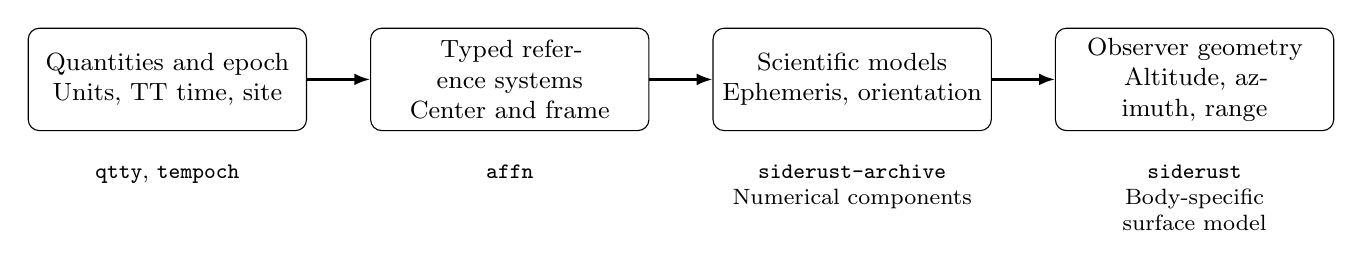
\begin{tikzpicture}[
  node distance=8mm,
  stage/.style={draw,rounded corners,align=center,text width=33mm,minimum height=13mm,font=\small},
  layer/.style={align=center,font=\footnotesize,text width=33mm},
  flow/.style={-{Latex[length=2mm]},thick}
]
\node[stage] (input) {Quantities and epoch\\Units, TT time, site};
\node[stage,right=of input] (reference) {Typed reference systems\\Center and frame};
\node[stage,right=of reference] (models) {Scientific models\\Ephemeris, orientation};
\node[stage,right=of models] (observable) {Observer geometry\\Altitude, azimuth, range};
\draw[flow] (input)--(reference);
\draw[flow] (reference)--(models);
\draw[flow] (models)--(observable);
\node[layer,below=3mm of input] {\texttt{qtty}, \texttt{tempoch}};
\node[layer,below=3mm of reference] {\texttt{affn}};
\node[layer,below=3mm of models] {\texttt{siderust-archive}\\Numerical components};
\node[layer,below=3mm of observable] {\texttt{siderust}\\Body-specific surface model};
\end{tikzpicture}

\caption{Scientific composition in a surface-observation workflow. Typed
quantities, epochs and reference systems connect ephemeris and orientation
models to observer-relative geometry. Reusable libraries supply the mechanisms;
the Siderust domain layer selects and combines the astronomical operations.
The diagram was prepared with AI-assisted TikZ authoring.}
\label{fig:architecture}
\end{figure*}

\subsection{Shared scientific representations}

\texttt{qtty} provides dimensional quantities with unit and scalar parameters.
Conversion changes the unit representation explicitly, while multiplication and
division construct compound quantities. \texttt{affn} provides generic Cartesian,
spherical and ellipsoidal containers, reference-frame and reference-center
traits, affine operators and conic geometry. \texttt{tempoch} supplies
scale-parameterized instants, durations, intervals and encoded epoch views.
Together, these libraries define the vocabulary shared by the scientific layers.

For example, a position uses quantities for its components and carries frame
and center markers through transformations. An epoch remains typed when passed
to an orientation model. The result of a local observation retains its observer
parameters while presenting altitude, azimuth and range as quantities.
This arrangement supports consistent reuse: the geometry library handles
coordinate structure, the time library handles temporal representation, and
the domain layer interprets both for a particular astronomical calculation.

\subsection{Models, numerical components and domain composition}

\texttt{siderust-archive} supplies scientific datasets, manifests, checksums
and generated accessors. Analytical ephemerides and time conversions consume
these data through their respective implementations. \texttt{cheby} supplies
Chebyshev approximation and interpolation; \texttt{keplerian} supplies
central-force mechanics, conic propagation and Lambert solvers;
\texttt{principia} supplies numerical dynamics, integration and variational
equations; and \texttt{optica} supplies optical and radiometric primitives.
These components can be reused independently or assembled by the domain crate
(Table~\ref{tab:crate-products}).

The \texttt{siderust} crate adds celestial bodies, observatories, astronomical
transformations, analytical and runtime ephemerides, observing-event searches
and feature-gated orbital workflows. Generic surface observers illustrate
this division particularly well: a common projection pipeline operates on a
body-specific reference surface and orientation provider. Extending the
observer model therefore reuses the quantity, epoch and geometry layers
alongside the local-horizon calculation.
This separates two extension tasks: a new surface model supplies scientific
parameters, while the existing projection consumes the shared typed geometry.
The boundary cases described in Section~\ref{sec:evaluation} examine this
separation without changing the underlying orientation or ephemeris implementation.

\begin{table}[!tbp]
\centering
\caption{Reusable components and their role in scientific composition. Exact
versions and licensing terms are available from the published software releases.}
\label{tab:crate-products}
\footnotesize
\begin{tabularx}{\columnwidth}{@{}lY@{}}
\toprule
Component & Scientific responsibility \\
\midrule
\texttt{qtty} & Quantities, units and dimensional arithmetic \\
\texttt{affn} & Geometry, coordinate containers, frames and centers \\
\texttt{tempoch} & Epochs, time scales, durations and conversions \\
\texttt{siderust-archive} & Scientific datasets and provenance \\
\texttt{cheby} & Approximation, interpolation and calculus \\
\texttt{keplerian} & Analytic orbital mechanics and transfers \\
\texttt{principia} & Numerical dynamics and state transport \\
\texttt{optica} & Optical and radiometric operations \\
\texttt{siderust} & Astronomical models and integrated workflows \\
\bottomrule
\end{tabularx}
\end{table}

\subsection{Memory safety and scientific semantics}

Rust's ownership, borrowing and lifetime rules provide the memory and sharing
foundation for these components. Safe Rust prevents important classes of
invalid memory access and data races, assuming sound implementations of the
unsafe abstractions on which it relies \cite{rustbook,rustbelt2018}.
Siderust adds domain-level structure: unit, scale, frame and center types
constrain scientific operations, while fallible constructors and explicit
errors handle value-dependent conditions.

The released domain crate inherits a workspace
\texttt{unsafe\_code = "forbid"} lint. Its FFI package has a separate lint
configuration allowing unsafe code at the foreign boundary; dependencies have
their own implementation policies. This source policy complements API design
and testing. Scientific validity additionally depends on choosing suitable
models, data and inputs, as discussed in Section~9.

\section{Scientific Interfaces and Operations}

Astronomical operations in Siderust combine typed quantities, epochs and
coordinate containers. A transformation receives the scientific context it
needs and returns a value with the resulting representation. The listings
below are included directly from executable sources, all checked against the
published v0.16.0 dependency graph during CI.

\subsection{Quantities and units}

\texttt{qtty} represents a quantity as \texttt{Quantity<U,S>}, where
\texttt{U} identifies the unit and \texttt{S} the scalar. Compatible
conversions are explicit, and multiplication or division constructs compound
units. This lets an application compute a velocity directly from a distance and an
elapsed time, with the compound unit carried by the result.

\lstinputlisting[float=tbp,caption={Computing a velocity from typed distance and duration quantities.},label={lst:qtty}]{../examples/src/bin/qtty.rs}

The local \texttt{Speed} alias names an existing velocity type; it introduces
neither a new nominal type nor an additional guarantee. We use such aliases
in applications to shorten notation while retaining the unit parameters.

Dimensional checking supports these operations automatically. Higher layers
add domain distinctions such as longitude and azimuth where their roles differ
scientifically, since a common angle unit alone does not distinguish them.

\subsection{Astronomical time}

\texttt{tempoch} represents an instant as a scale- and encoding-parameterized
\texttt{Time}. Subtracting two compatible instants produces a duration, and
shifting an instant by a duration produces another instant. JD, MJD, Unix, GPS,
and J2000-second markers are conversion targets rather than unlabelled numeric
epochs.

\lstinputlisting[float=tbp,caption={Typed time-scale and encoding conversion using \texttt{tempoch}.},label={lst:tempoch}]{../examples/src/bin/tempoch.rs}

UTC conversion uses the active UTC--TAI table. UT1 conversion requires an Earth-orientation or
$\Delta T$ context, whose source, interpolation policy and coverage interval
are part of the evaluated configuration \cite{iers2010}. The context exposes the available interval; callers of the evaluated EOP
lookup must additionally check its exact upper bound because of the endpoint
defect documented in Section~8.

\subsection{Coordinates, frames, and centers}

\texttt{affn} defines \texttt{Position<C,F,U>}, where \texttt{C} is the
reference center, \texttt{F} the frame, and \texttt{U} the length unit.
A position transformation changes its frame or center marker explicitly.
Directions carry orientation independently of an origin, making them suitable
for distance-free pointing operations. Incompatible markers are checked when
values are combined.

Reference-center types may carry runtime parameters. In the evaluated snapshot,
\texttt{Topocentric} uses a \texttt{Geodetic<ECEF>} site as its parameter type.
\texttt{Bodycentric} instead uses a \texttt{BodycentricParams} value containing
an elliptic orbit, its reference center, and a gravitational parameter.
Coordinates with the same center type can therefore still carry different
parameters. Cartesian position subtraction is available as an operator only for
centers whose parameter type is \texttt{()}. For parameterized centers,
\texttt{checked\_sub} returns an error when the stored values differ.
The accompanying tests exercise both matching and mismatched sites.
Transform methods preserve or explicitly replace the
stored parameters. Site values identify the geometric observer; external station metadata and
site epochs are managed by the application.

\subsection{Generic surface observers}
\label{sec:surface}

We generalize surface observers through
\texttt{SurfaceSite<B>}. A body model associates \texttt{B} with a center,
body-fixed frame and default reference surface. The same transformation
infrastructure then serves lunar, terrestrial and other supported surfaces.
The body parameter is static; longitude, latitude, height, surface parameters
and their admissibility are checked values. Planetographic latitude identifies
the ellipsoid normal, whereas planetocentric latitude selects a radial
intersection with the surface. Height and local vertical follow the surface
normal in both cases; on a sphere, these latitude definitions coincide.

A finite position is translated to the body's center and the observer's
location is subtracted before local angular extraction, retaining range and
parallax. A distance-free direction undergoes rotation only. The local east--north--up
basis is right-handed; the public \texttt{Horizontal} Cartesian ordering is
north, east, up, consistent with azimuth measured from north through east.
The component order is explicit at the public interface.

The high-level direction observation retains both \texttt{B} and the site
values. Checked inversion rejects a different site, while a different body
is rejected by the type system. Low-level \texttt{Direction<Horizontal>}
values do not themselves retain the observer. The epoch and orientation context are supplied explicitly to each observation.
This design connects static body identity with value-dependent observer geometry.

\subsection{Astronomy workflows}

The domain crate supplies transforms, ephemerides, bodies, observatories,
altitude calculations, observing-event searches, and feature-gated dynamics
workflows. Analytical planetary and lunar paths use archive-backed VSOP87 and
ELP2000-82B data \cite{bretagnon1988vsop87,chapront1983elp2000}; runtime paths
load externally supplied JPL/NAIF BSP kernels \cite{naifspk,park2021de440}.

\lstinputlisting[float=tbp,caption={Runtime SPK-backed ephemeris access. The application supplies the BSP file at execution time.},label={lst:runtime-eph}]{../examples/src/bin/runtime_ephemeris.rs}

The common ephemeris interface lets an application select an analytical model
or a supplied SPK kernel through common frame and center types. Their physical
frame realizations are specified in Section~7.1.
The evaluation records that choice together with the body definition and
correction mode, connecting each result to its scientific model.


\subsection{Three levels of scientific contract}

Static contracts constrain compatible unit, frame, center, scale and observer-body
parameters. Dynamic contracts validate values sharing those types: two sites
can have different coordinates, a vector can be degenerate, and a query can exceed
a dataset's coverage. Scientific contracts concern the intended observable:
ephemeris choice, frame realization, geometric or apparent corrections, body
orientation, surface definition and data accuracy. These require model selection
and numerical validation rather than type checking.

Table~\ref{tab:guarantees} summarizes the executed static and dynamic controls.
The semantic matrix below summarizes the observed enforcement mechanisms and
outcomes for the evaluated public APIs.
The evaluation included five compiler-failure controls; runtime cases covered
nonfinite values, invalid latitude, a surface-normal singularity, zero direction
and mismatched observers. Dataset coverage was examined separately, revealing
the EOP and exact SPK endpoint behaviors described in the results.

\begin{table*}[!tbp]
\centering
\caption{Static and runtime semantic controls observed with published v0.16.0.
Scientific model adequacy is assessed by numerical references, not by these contracts.}
\label{tab:guarantees}
\footnotesize
\begin{tabularx}{\textwidth}{@{}YYYY@{}}
\toprule
Constraint & API & Mechanism & Outcome \\
\midrule
observer\_\allowbreak{}body & horizontal\_\allowbreak{}observation\_\allowbreak{}to\_\allowbreak{}direction$<$B$>$ & static type/trait compatibility & rejected: E0308 \\
center & Position$<$C,F,U$>$ subtraction & static type/trait compatibility & rejected: E0277 \\
dimension & Quantity$<$U,S$>$ addition & static type/trait compatibility & rejected: E0308 \\
frame & Position$<$C,F,U$>$ subtraction & static type/trait compatibility & rejected: E0277 \\
scale & gmst\_\allowbreak{}iau2006(UT1,TT) & static type/trait compatibility & rejected: E0308 \\
observer values & Position::checked\_\allowbreak{}sub & runtime Result & valid accepted; invalid rejected \\
finite inputs / surface domain & SurfaceSite::new & runtime Result & valid accepted; invalid rejected \\
zero/nonfinite direction & SurfaceHorizontalExt::observe\_\allowbreak{}direction & runtime Result & valid accepted; invalid rejected \\
surface observer values & horizontal\_\allowbreak{}observation\_\allowbreak{}to\_\allowbreak{}direction & runtime Result & valid accepted; invalid rejected \\
\bottomrule
\end{tabularx}

\end{table*}

\section{Language Interfaces}

External applications access selected scientific operations through
C-compatible entry points in
\texttt{qtty-ffi}, \texttt{tempoch-ffi} and \texttt{siderust-ffi}. Values,
handles and explicit status codes connect foreign applications to the Rust
implementation. This architecture centralizes scientific computation while
allowing host-language adapters to provide their own application interfaces.

Rust trait constraints are enforced within the Rust implementation; a foreign
boundary expresses its contract through value validation, ownership rules and
error translation. The numerical results reported here evaluate the Rust APIs.
The available FFI source interfaces are distinct from separately maintained
C++, Python and JavaScript/WASM adapters. Testing corresponding host workflows
and freezing wrapper releases are further steps toward broader cross-language
deployment.

\section{Applications in Observer Geometry}
\label{sec:application}

\subsection{A terrestrial viewing window}

For the terrestrial application, we determine when a target exceeds
$30^\circ$ altitude during 2025 January 1 UTC at a site with longitude $1.5^\circ$ east, geodetic latitude $42^\circ$
north and zero ellipsoidal height. The prescribed direction has right ascension
$120^\circ$ and declination $20^\circ$ in the true equator and equinox of date.
It defines a reproducible pointing scenario with fixed angular coordinates.

The calculation constructs a UTC epoch, converts it to TT and calls
\texttt{to\_horizontal\_precise} with a separately typed UT1 epoch and the
site. We prescribe $\mathrm{UT1}-\mathrm{UTC}=0$ for this example and sample
\ViewingSampleCount{} epochs at five-minute spacing, including both day
endpoints. Selection above the threshold produces \ViewingSelectedCount{}
samples spanning \ViewingSpans{} UTC.
Figure~\ref{fig:viewing-window} displays the complete grid.
These are selected sample spans; threshold crossings lie between adjacent
five-minute samples and are not root-refined rise or set times.

The independent reduction combines ERFA \texttt{gst06a} and \texttt{hd2ae}
with the same inputs. The maximum altitude difference is below
$\AltitudeBound$ degrees. Site geometry, angular units, frame and time scales
remain explicit throughout the selection, illustrating how a simple planning
operation composes several scientific representations.

\begin{figure}[!tbp]
\centering
% Published figure with the original 289 altitude samples.
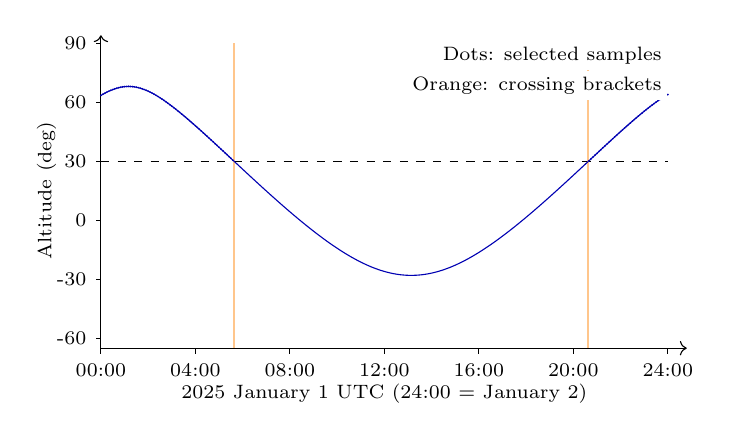
\begin{tikzpicture}[x=0.30cm,y=0.025cm,font=\scriptsize]
\draw[->] (0,-65) -- (24.8,-65);
\draw[->] (0,-65) -- (0,94);
\draw (0,-65) -- (0,-68) node[below] {00:00};
\draw (4,-65) -- (4,-68) node[below] {04:00};
\draw (8,-65) -- (8,-68) node[below] {08:00};
\draw (12,-65) -- (12,-68) node[below] {12:00};
\draw (16,-65) -- (16,-68) node[below] {16:00};
\draw (20,-65) -- (20,-68) node[below] {20:00};
\draw (24,-65) -- (24,-68) node[below] {24:00};
\draw (0,-60) -- (-0.2,-60) node[left] {-60};
\draw (0,-30) -- (-0.2,-30) node[left] {-30};
\draw (0,0) -- (-0.2,0) node[left] {0};
\draw (0,30) -- (-0.2,30) node[left] {30};
\draw (0,60) -- (-0.2,60) node[left] {60};
\draw (0,90) -- (-0.2,90) node[left] {90};
\node at (12,-88) {2025 January 1 UTC (24:00 = January 2)};
\node[rotate=90] at (-2.3,15) {Altitude (deg)};
\draw[dashed] (0,30) -- (24,30);
\fill[orange!45] (5.583333,-65) rectangle (5.666667,90);
\fill[orange!45] (20.583333,-65) rectangle (20.666667,90);
\draw[blue!70!black,thin] plot coordinates {(0.000000,63.4435271617)
(0.083333,64.0208957836)
(0.166667,64.5676418220)
(0.250000,65.0816724668)
(0.333333,65.5608515973)
(0.416667,66.0030245915)
(0.500000,66.4060497416)
(0.583333,66.7678340287)
(0.666667,67.0863744955)
(0.750000,67.3598023271)
(0.833333,67.5864294475)
(0.916667,67.7647942559)
(1.000000,67.8937045183)
(1.083333,67.9722747745)
(1.166667,67.9999551928)
(1.250000,67.9765502258)
(1.333333,67.9022252932)
(1.416667,67.7775010753)
(1.500000,67.6032359699)
(1.583333,67.3805977984)
(1.666667,67.1110271663)
(1.750000,66.7961950380)
(1.833333,66.4379567207)
(1.916667,66.0383058597)
(2.000000,65.5993293631)
(2.083333,65.1231665398)
(2.166667,64.6119719575)
(2.250000,64.0678845878)
(2.333333,63.4930015171)
(2.416667,62.8893577305)
(2.500000,62.2589110067)
(2.583333,61.6035304663)
(2.666667,60.9249902398)
(2.750000,60.2249649807)
(2.833333,59.5050294153)
(2.916667,58.7666584587)
(3.000000,58.0112303998)
(3.083333,57.2400297538)
(3.166667,56.4542518664)
(3.250000,55.6550080506)
(3.333333,54.8433299273)
(3.416667,54.0201754650)
(3.500000,53.1864332639)
(3.583333,52.3429284700)
(3.666667,51.4904267249)
(3.750000,50.6296396814)
(3.833333,49.7612285601)
(3.916667,48.8858085685)
(4.000000,48.0039530645)
(4.083333,47.1161962660)
(4.166667,46.2230374660)
(4.250000,45.3249430982)
(4.333333,44.4223504729)
(4.416667,43.5156693680)
(4.500000,42.6052853429)
(4.583333,41.6915610409)
(4.666667,40.7748385258)
(4.750000,39.8554414624)
(4.833333,38.9336759153)
(4.916667,38.0098328570)
(5.000000,37.0841885763)
(5.083333,36.1570069523)
(5.166667,35.2285396403)
(5.250000,34.2990281507)
(5.333333,33.3687039774)
(5.416667,32.4377898909)
(5.500000,31.5065011647)
(5.583333,30.5750454868)
(5.666667,29.6436246882)
(5.750000,28.7124344188)
(5.833333,27.7816657754)
(5.916667,26.8515048884)
(6.000000,25.9221344661)
(6.083333,24.9937334329)
(6.166667,24.0664777832)
(6.250000,23.1405414041)
(6.333333,22.2160956302)
(6.416667,21.2933106372)
(6.500000,20.3723548301)
(6.583333,19.4533961929)
(6.666667,18.5366016441)
(6.750000,17.6221383491)
(6.833333,16.7101731727)
(6.916667,15.8008733490)
(7.000000,14.8944071351)
(7.083333,13.9909432366)
(7.166667,13.0906520487)
(7.250000,12.1937049479)
(7.333333,11.3002755098)
(7.416667,10.4105387931)
(7.500000,9.5246725362)
(7.583333,8.6428565544)
(7.666667,7.7652733273)
(7.750000,6.8921085714)
(7.833333,6.0235506347)
(7.916667,5.1597916457)
(8.000000,4.3010267884)
(8.083333,3.4474554314)
(8.166667,2.5992804039)
(8.250000,1.7567091034)
(8.333333,0.9199528843)
(8.416667,0.0892275835)
(8.500000,-0.7352459745)
(8.583333,-1.5532425877)
(8.666667,-2.3645316321)
(8.750000,-3.1688777875)
(8.833333,-3.9660400244)
(8.916667,-4.7557723350)
(9.000000,-5.5378227561)
(9.083333,-6.3119340052)
(9.166667,-7.0778430627)
(9.250000,-7.8352807890)
(9.333333,-8.5839725781)
(9.416667,-9.3236375011)
(9.500000,-10.0539890853)
(9.583333,-10.7747345195)
(9.666667,-11.4855754599)
(9.750000,-12.1862073066)
(9.833333,-12.8763199519)
(9.916667,-13.5555975970)
(10.000000,-14.2237186267)
(10.083333,-14.8803564220)
(10.166667,-15.5251788585)
(10.250000,-16.1578492681)
(10.333333,-16.7780260458)
(10.416667,-17.3853636735)
(10.500000,-17.9795124462)
(10.583333,-18.5601194879)
(10.666667,-19.1268289909)
(10.750000,-19.6792825410)
(10.833333,-20.2171202435)
(10.916667,-20.7399807837)
(11.000000,-21.2475027120)
(11.083333,-21.7393246469)
(11.166667,-22.2150866360)
(11.250000,-22.6744304993)
(11.333333,-23.1170012024)
(11.416667,-23.5424476244)
(11.500000,-23.9504234112)
(11.583333,-24.3405884240)
(11.666667,-24.7126093914)
(11.750000,-25.0661614482)
(11.833333,-25.4009288788)
(11.916667,-25.7166066539)
(12.000000,-26.0129012368)
(12.083333,-26.2895320492)
(12.166667,-26.5462324841)
(12.250000,-26.7827509451)
(12.333333,-26.9988521799)
(12.416667,-27.1943180835)
(12.500000,-27.3689489350)
(12.583333,-27.5225641293)
(12.666667,-27.6550032337)
(12.750000,-27.7661266091)
(12.833333,-27.8558162366)
(12.916667,-27.9239762468)
(13.000000,-27.9705333940)
(13.083333,-27.9954374902)
(13.166667,-27.9986616147)
(13.250000,-27.9802022810)
(13.333333,-27.9400794512)
(13.416667,-27.8783364128)
(13.500000,-27.7950395967)
(13.583333,-27.6902781846)
(13.666667,-27.5641636642)
(13.750000,-27.4168293287)
(13.833333,-27.2484294849)
(13.916667,-27.0591388513)
(14.000000,-26.8491515323)
(14.083333,-26.6186802999)
(14.166667,-26.3679553814)
(14.250000,-26.0972236642)
(14.333333,-25.8067473794)
(14.416667,-25.4968030680)
(14.500000,-25.1676805714)
(14.583333,-24.8196815731)
(14.666667,-24.4531187859)
(14.750000,-24.0683144183)
(14.833333,-23.6655994194)
(14.916667,-23.2453119394)
(15.000000,-22.8077966611)
(15.083333,-22.3534033460)
(15.166667,-21.8824859662)
(15.250000,-21.3954019208)
(15.333333,-20.8925106526)
(15.416667,-20.3741732843)
(15.500000,-19.8407512467)
(15.583333,-19.2926060544)
(15.666667,-18.7300980092)
(15.750000,-18.1535861187)
(15.833333,-17.5634269580)
(15.916667,-16.9599743270)
(16.000000,-16.3435789939)
(16.083333,-15.7145876679)
(16.166667,-15.0733432546)
(16.250000,-14.4201838224)
(16.333333,-13.7554429783)
(16.416667,-13.0794488981)
(16.500000,-12.3925248115)
(16.583333,-11.6949881827)
(16.666667,-10.9871508231)
(16.750000,-10.2693190645)
(16.833333,-9.5417930036)
(16.916667,-8.8048672155)
(17.000000,-8.0588299420)
(17.083333,-7.3039638768)
(17.166667,-6.5405453830)
(17.250000,-5.7688453406)
(17.333333,-4.9891284902)
(17.416667,-4.2016538102)
(17.500000,-3.4066749286)
(17.583333,-2.6044394860)
(17.666667,-1.7951901061)
(17.750000,-0.9791636638)
(17.833333,-0.1565922937)
(17.916667,0.6722973371)
(18.000000,1.5072829878)
(18.083333,2.3481474557)
(18.166667,3.1946780727)
(18.250000,4.0466661828)
(18.333333,4.9039077537)
(18.416667,5.7662022718)
(18.500000,6.6333534668)
(18.583333,7.5051681854)
(18.666667,8.3814571158)
(18.750000,9.2620336423)
(18.833333,10.1467144504)
(18.916667,11.0353189566)
(19.000000,11.9276687229)
(19.083333,12.8235880603)
(19.166667,13.7229028351)
(19.250000,14.6254411860)
(19.333333,15.5310323093)
(19.416667,16.4395071686)
(19.500000,17.3506972578)
(19.583333,18.2644351767)
(19.666667,19.1805539820)
(19.750000,20.0988865201)
(19.833333,21.0192659789)
(19.916667,21.9415245797)
(20.000000,22.8654942264)
(20.083333,23.7910051615)
(20.166667,24.7178865833)
(20.250000,25.6459652591)
(20.333333,26.5750659779)
(20.416667,27.5050107353)
(20.500000,28.4356178888)
(20.583333,29.3667025295)
(20.666667,30.2980749482)
(20.750000,31.2295410608)
(20.833333,32.1609007943)
(20.916667,33.0919484245)
(21.000000,34.0224708642)
(21.083333,34.9522477695)
(21.166667,35.8810503332)
(21.250000,36.8086400129)
(21.333333,37.7347684271)
(21.416667,38.6591753025)
(21.500000,39.5815883170)
(21.583333,40.5017208575)
(21.666667,41.4192716475)
(21.750000,42.3339222756)
(21.833333,43.2453364411)
(21.916667,44.1531578180)
(22.000000,45.0570077691)
(22.083333,45.9564840983)
(22.166667,46.8511577953)
(22.250000,47.7405715094)
(22.333333,48.6242358801)
(22.416667,49.5016275458)
(22.500000,50.3721850036)
(22.583333,51.2353059801)
(22.666667,52.0903433500)
(22.750000,52.9366007967)
(22.833333,53.7733293388)
(22.916667,54.5997218855)
(23.000000,55.4149093561)
(23.083333,56.2179548120)
(23.166667,57.0078492048)
(23.250000,57.7835053290)
(23.333333,58.5437534397)
(23.416667,59.2873360127)
(23.500000,60.0129029646)
(23.583333,60.7190085406)
(23.666667,61.4041077478)
(23.750000,62.0665557374)
(23.833333,62.7046075846)
(23.916667,63.3164219447)
(24.000000,63.9000663521)};
\fill[blue!70!black] (0.000000,63.4435271617) circle[radius=0.35pt];
\fill[blue!70!black] (0.083333,64.0208957836) circle[radius=0.35pt];
\fill[blue!70!black] (0.166667,64.5676418220) circle[radius=0.35pt];
\fill[blue!70!black] (0.250000,65.0816724668) circle[radius=0.35pt];
\fill[blue!70!black] (0.333333,65.5608515973) circle[radius=0.35pt];
\fill[blue!70!black] (0.416667,66.0030245915) circle[radius=0.35pt];
\fill[blue!70!black] (0.500000,66.4060497416) circle[radius=0.35pt];
\fill[blue!70!black] (0.583333,66.7678340287) circle[radius=0.35pt];
\fill[blue!70!black] (0.666667,67.0863744955) circle[radius=0.35pt];
\fill[blue!70!black] (0.750000,67.3598023271) circle[radius=0.35pt];
\fill[blue!70!black] (0.833333,67.5864294475) circle[radius=0.35pt];
\fill[blue!70!black] (0.916667,67.7647942559) circle[radius=0.35pt];
\fill[blue!70!black] (1.000000,67.8937045183) circle[radius=0.35pt];
\fill[blue!70!black] (1.083333,67.9722747745) circle[radius=0.35pt];
\fill[blue!70!black] (1.166667,67.9999551928) circle[radius=0.35pt];
\fill[blue!70!black] (1.250000,67.9765502258) circle[radius=0.35pt];
\fill[blue!70!black] (1.333333,67.9022252932) circle[radius=0.35pt];
\fill[blue!70!black] (1.416667,67.7775010753) circle[radius=0.35pt];
\fill[blue!70!black] (1.500000,67.6032359699) circle[radius=0.35pt];
\fill[blue!70!black] (1.583333,67.3805977984) circle[radius=0.35pt];
\fill[blue!70!black] (1.666667,67.1110271663) circle[radius=0.35pt];
\fill[blue!70!black] (1.750000,66.7961950380) circle[radius=0.35pt];
\fill[blue!70!black] (1.833333,66.4379567207) circle[radius=0.35pt];
\fill[blue!70!black] (1.916667,66.0383058597) circle[radius=0.35pt];
\fill[blue!70!black] (2.000000,65.5993293631) circle[radius=0.35pt];
\fill[blue!70!black] (2.083333,65.1231665398) circle[radius=0.35pt];
\fill[blue!70!black] (2.166667,64.6119719575) circle[radius=0.35pt];
\fill[blue!70!black] (2.250000,64.0678845878) circle[radius=0.35pt];
\fill[blue!70!black] (2.333333,63.4930015171) circle[radius=0.35pt];
\fill[blue!70!black] (2.416667,62.8893577305) circle[radius=0.35pt];
\fill[blue!70!black] (2.500000,62.2589110067) circle[radius=0.35pt];
\fill[blue!70!black] (2.583333,61.6035304663) circle[radius=0.35pt];
\fill[blue!70!black] (2.666667,60.9249902398) circle[radius=0.35pt];
\fill[blue!70!black] (2.750000,60.2249649807) circle[radius=0.35pt];
\fill[blue!70!black] (2.833333,59.5050294153) circle[radius=0.35pt];
\fill[blue!70!black] (2.916667,58.7666584587) circle[radius=0.35pt];
\fill[blue!70!black] (3.000000,58.0112303998) circle[radius=0.35pt];
\fill[blue!70!black] (3.083333,57.2400297538) circle[radius=0.35pt];
\fill[blue!70!black] (3.166667,56.4542518664) circle[radius=0.35pt];
\fill[blue!70!black] (3.250000,55.6550080506) circle[radius=0.35pt];
\fill[blue!70!black] (3.333333,54.8433299273) circle[radius=0.35pt];
\fill[blue!70!black] (3.416667,54.0201754650) circle[radius=0.35pt];
\fill[blue!70!black] (3.500000,53.1864332639) circle[radius=0.35pt];
\fill[blue!70!black] (3.583333,52.3429284700) circle[radius=0.35pt];
\fill[blue!70!black] (3.666667,51.4904267249) circle[radius=0.35pt];
\fill[blue!70!black] (3.750000,50.6296396814) circle[radius=0.35pt];
\fill[blue!70!black] (3.833333,49.7612285601) circle[radius=0.35pt];
\fill[blue!70!black] (3.916667,48.8858085685) circle[radius=0.35pt];
\fill[blue!70!black] (4.000000,48.0039530645) circle[radius=0.35pt];
\fill[blue!70!black] (4.083333,47.1161962660) circle[radius=0.35pt];
\fill[blue!70!black] (4.166667,46.2230374660) circle[radius=0.35pt];
\fill[blue!70!black] (4.250000,45.3249430982) circle[radius=0.35pt];
\fill[blue!70!black] (4.333333,44.4223504729) circle[radius=0.35pt];
\fill[blue!70!black] (4.416667,43.5156693680) circle[radius=0.35pt];
\fill[blue!70!black] (4.500000,42.6052853429) circle[radius=0.35pt];
\fill[blue!70!black] (4.583333,41.6915610409) circle[radius=0.35pt];
\fill[blue!70!black] (4.666667,40.7748385258) circle[radius=0.35pt];
\fill[blue!70!black] (4.750000,39.8554414624) circle[radius=0.35pt];
\fill[blue!70!black] (4.833333,38.9336759153) circle[radius=0.35pt];
\fill[blue!70!black] (4.916667,38.0098328570) circle[radius=0.35pt];
\fill[blue!70!black] (5.000000,37.0841885763) circle[radius=0.35pt];
\fill[blue!70!black] (5.083333,36.1570069523) circle[radius=0.35pt];
\fill[blue!70!black] (5.166667,35.2285396403) circle[radius=0.35pt];
\fill[blue!70!black] (5.250000,34.2990281507) circle[radius=0.35pt];
\fill[blue!70!black] (5.333333,33.3687039774) circle[radius=0.35pt];
\fill[blue!70!black] (5.416667,32.4377898909) circle[radius=0.35pt];
\fill[blue!70!black] (5.500000,31.5065011647) circle[radius=0.35pt];
\fill[blue!70!black] (5.583333,30.5750454868) circle[radius=0.35pt];
\fill[blue!70!black] (20.666667,30.2980749482) circle[radius=0.35pt];
\fill[blue!70!black] (20.750000,31.2295410608) circle[radius=0.35pt];
\fill[blue!70!black] (20.833333,32.1609007943) circle[radius=0.35pt];
\fill[blue!70!black] (20.916667,33.0919484245) circle[radius=0.35pt];
\fill[blue!70!black] (21.000000,34.0224708642) circle[radius=0.35pt];
\fill[blue!70!black] (21.083333,34.9522477695) circle[radius=0.35pt];
\fill[blue!70!black] (21.166667,35.8810503332) circle[radius=0.35pt];
\fill[blue!70!black] (21.250000,36.8086400129) circle[radius=0.35pt];
\fill[blue!70!black] (21.333333,37.7347684271) circle[radius=0.35pt];
\fill[blue!70!black] (21.416667,38.6591753025) circle[radius=0.35pt];
\fill[blue!70!black] (21.500000,39.5815883170) circle[radius=0.35pt];
\fill[blue!70!black] (21.583333,40.5017208575) circle[radius=0.35pt];
\fill[blue!70!black] (21.666667,41.4192716475) circle[radius=0.35pt];
\fill[blue!70!black] (21.750000,42.3339222756) circle[radius=0.35pt];
\fill[blue!70!black] (21.833333,43.2453364411) circle[radius=0.35pt];
\fill[blue!70!black] (21.916667,44.1531578180) circle[radius=0.35pt];
\fill[blue!70!black] (22.000000,45.0570077691) circle[radius=0.35pt];
\fill[blue!70!black] (22.083333,45.9564840983) circle[radius=0.35pt];
\fill[blue!70!black] (22.166667,46.8511577953) circle[radius=0.35pt];
\fill[blue!70!black] (22.250000,47.7405715094) circle[radius=0.35pt];
\fill[blue!70!black] (22.333333,48.6242358801) circle[radius=0.35pt];
\fill[blue!70!black] (22.416667,49.5016275458) circle[radius=0.35pt];
\fill[blue!70!black] (22.500000,50.3721850036) circle[radius=0.35pt];
\fill[blue!70!black] (22.583333,51.2353059801) circle[radius=0.35pt];
\fill[blue!70!black] (22.666667,52.0903433500) circle[radius=0.35pt];
\fill[blue!70!black] (22.750000,52.9366007967) circle[radius=0.35pt];
\fill[blue!70!black] (22.833333,53.7733293388) circle[radius=0.35pt];
\fill[blue!70!black] (22.916667,54.5997218855) circle[radius=0.35pt];
\fill[blue!70!black] (23.000000,55.4149093561) circle[radius=0.35pt];
\fill[blue!70!black] (23.083333,56.2179548120) circle[radius=0.35pt];
\fill[blue!70!black] (23.166667,57.0078492048) circle[radius=0.35pt];
\fill[blue!70!black] (23.250000,57.7835053290) circle[radius=0.35pt];
\fill[blue!70!black] (23.333333,58.5437534397) circle[radius=0.35pt];
\fill[blue!70!black] (23.416667,59.2873360127) circle[radius=0.35pt];
\fill[blue!70!black] (23.500000,60.0129029646) circle[radius=0.35pt];
\fill[blue!70!black] (23.583333,60.7190085406) circle[radius=0.35pt];
\fill[blue!70!black] (23.666667,61.4041077478) circle[radius=0.35pt];
\fill[blue!70!black] (23.750000,62.0665557374) circle[radius=0.35pt];
\fill[blue!70!black] (23.833333,62.7046075846) circle[radius=0.35pt];
\fill[blue!70!black] (23.916667,63.3164219447) circle[radius=0.35pt];
\fill[blue!70!black] (24.000000,63.9000663521) circle[radius=0.35pt];
\node[anchor=north east,fill=white,inner sep=2pt] at (24,91) {Dots: selected samples};
\node[anchor=north east,fill=white,inner sep=2pt] at (24,76) {Orange: crossing brackets};
\end{tikzpicture}

\caption{All 289 terrestrial altitude samples. The line joins sampled values;
dots mark the 109 selected samples, and the dashed line is the $30^\circ$
threshold. Shaded five-minute brackets contain the two crossings; no refined
event times are implied. The plot is based on the 289 evaluated samples;
its plotting code was AI-assisted.}
\label{fig:viewing-window}
\end{figure}

\subsection{Earth seen from a lunar surface site}
\label{sec:lunar-example}

Our second application computes Earth's geometric altitude, azimuth and range
from a lunar station at $20^\circ$ east longitude and $-3.5^\circ$
planetocentric latitude at TT JD $2460000.5$. The observer lies on the
$1737.4$ km reference sphere, so the local vertical is radial. This calculation
combines a finite-distance ephemeris target with the generic surface-observer
architecture introduced in Siderust v0.16.0.

Listing~\ref{lst:moon-surface} loads the DE440s kernel and evaluates the Moon's
geocentric position. Reversing that vector gives Earth's selenocentric position
in the same mean-ecliptic J2000 frame. The explicit \texttt{EarthFromMoon}
alias retains the target's center, frame and length unit. The surface API
rotates the target into the lunar body-fixed frame, subtracts the observer
position and projects the resulting line of sight onto the local horizon.
The target remains a position throughout, preserving range and parallax.
Writing $\boldsymbol r$ for Earth's selenocentric inertial vector,
$R$ for the inertial-to-body-fixed rotation, and $\boldsymbol s$ for the
body-fixed site, the local vector is
\begin{equation}
 \boldsymbol\ell =
 \begin{pmatrix}\boldsymbol n^{\mathsf T}\\
                 \boldsymbol e^{\mathsf T}\\
                 \boldsymbol u^{\mathsf T}\end{pmatrix}
 (R\boldsymbol r-\boldsymbol s),
\end{equation}
where $\boldsymbol n$, $\boldsymbol e$ and $\boldsymbol u$ are the local
north, east and up unit vectors. Range is $\lVert\boldsymbol\ell\rVert$;
altitude is $\operatorname{atan2}(\ell_u,\sqrt{\ell_n^2+\ell_e^2})$
and azimuth is $\operatorname{atan2}(\ell_e,\ell_n)$ modulo $2\pi$.
This ordering makes the observer subtraction and azimuth signs explicit.

\lstinputlisting[float=tbp,caption={Earth from a lunar observer using published v0.16.0 APIs. The argument supplies the DE440s BSP file. The output is altitude and azimuth in degrees, followed by range in kilometres.},label={lst:moon-surface}]{../examples/src/bin/earth_from_moon.rs}

The result is altitude $\EarthAltitude^\circ$, azimuth $\EarthAzimuth^\circ$ and range
$\EarthRange$ km. An independent CSPICE reduction of the same ephemeris and
surface geometry agrees within $\EarthAngleBound$ degrees and
$\EarthRangeBound$ km. The corresponding Moon-center direction has altitude
$\CentreAltitude^\circ$: observer displacement changes the altitude by about
$\EarthParallax^\circ$. This difference demonstrates why a nearby target requires
finite-distance geometry. The selected Earth position is above the horizon;
the example computes a pointing state rather than an Earthrise event.

We use the analytical text-PCK \texttt{IAU\_MOON} orientation,
which approximates the lunar mean-Earth/polar-axis convention and is exposed as \texttt{MoonIauMeanEarth}. Its periodic arguments use
TDB converted from the supplied TT epoch. This model is distinct from
DE-specific \texttt{MOON\_PA} and binary-PCK \texttt{MOON\_ME} realizations
\cite{archinal2011,naiflunarframes}. Azimuth increases from north through east.
Both applications compute geometric quantities, with atmospheric refraction,
light time, aberration, deflection and terrain masking omitted. These model
choices define the observables used in the comparisons.

\section{Experimental Method}
\label{sec:evaluation}

Published Siderust v0.16.0 is evaluated through independent numerical comparisons,
executable controls and paired arithmetic measurements. The evaluated package
corresponds to release revision \texttt{3e0069d3}. A committed Cargo lockfile
pins the published crate versions used by the accompanying executable examples,
which supply every printed listing. Reference methods, test inputs and tolerances
are described below. Original raw measurements, independent reference
fixtures and reproduction scripts are preserved in a separate, version-pinned
supplement branch rather than in the publication-source tree.
The full experimental execution infrastructure is not required for building the manuscript.

\subsection{Reference transformations and ephemerides}

We compare time and frame operations with ERFA 2.0.1 through PyERFA 2.0.1.5,
and kernel-backed positions with CSPICE N0067 through SpiceyPy 6.0.0.
Earth rotation angle, IAU 2006 GMST, mean obliquity and the IAU 2006/2000A
bias--precession--nutation matrix are evaluated at 1,000 deterministic Julian
dates $2451545-36525+73.125i$, $0\leq i<1000$. These isolated rotation tests
supply equal numerical TT and UT1 dates as controlled arguments. Ten UTC dates
from 1972 to 2025 exercise UTC--TAI and UTC--TT around selected leap-second
changes; full-JD comparisons use a $50\,\mu$s tolerance.
A separate pinned feature graph enables runtime time-data loading for a compact
IERS extension: 13 civil UTC labels include the 1972, 2015 and 2016 inserted
seconds, and six epochs compare EOP-backed UT1, Earth rotation and GMST.
Independent ERFA two-part UTC quasi-JD references are converted to continuous
TAI, TT and UT1 before differencing. The native time interface retains split
seconds; scalar UTC JD is rejected during an inserted second.
IERS daily samples also test polar-motion values and leap-aware interpolation
of UT1--TAI across the 2016 step. The evaluation used fixed IERS inputs, documented coverage limits and
specified acceptance tolerances.

For ephemerides, we compare Earth heliocentric and Moon geocentric positions
with the same DE440s kernel \cite{park2021de440,naifspk}. The sample contains
1,000 eight-day-spaced TT epochs beginning at J2000 and one-second interior
points near both coverage endpoints. CSPICE converts TT to ET using the NAIF
leap-second kernel. ERFA's \texttt{ecm06} aligns the reference ICRF vectors
with Siderust's IAU 2006 mean-ecliptic J2000 convention; SPICE's
\texttt{ECLIPJ2000} uses a different obliquity. Exact endpoints and one-day
out-of-coverage requests are tested separately.

Acceptance bounds are $2\times10^{-11}$ rad for Earth rotation and GMST,
$10^{-14}$ rad for obliquity, $2\times10^{-12}$ per matrix element,
$2\times10^{-12}$ au for Earth and $2\times10^{-4}$ km for the Moon.
They measure implementation agreement with the specified references.
The analytical VSOP87A and ELP2000-82B outputs are compared separately with
DE440s as backend-output differences. VSOP87A retains its native dynamical
ecliptic and equinox of J2000; ELP2000-82B retains its dynamical ecliptic J2000
coordinates after the implemented Laskar rotation
\cite{bretagnon1988vsop87,chapront1988elp85}. Both are returned with the
\texttt{EclipticMeanJ2000} marker in v0.16.0, while the SPK path uses the
IAU 2006 realization above. The recorded comparison therefore includes
frame-realization effects as well as orbital-model differences.

For ephemeris positions, the residual is the Euclidean norm
\begin{equation}
 \Delta r=\left\|\boldsymbol r_{\mathrm{Siderust}}
                  -\boldsymbol r_{\mathrm{reference}}\right\|_2.
\end{equation}
Matrix residuals are maximum absolute element differences. Altitude and time
residuals are absolute scalar differences; azimuth differences are wrapped
to the shorter angular separation.

\subsection{Surface geometry and integrated observations}

The terrestrial application is evaluated on its complete 289-epoch grid.
Thirty lunar direction cases combine five epochs in TT spanning 1900--2050,
two sites and three ICRS directions. A fixed synthetic finite target gives
ten distinct epoch/site/target geometries, each executed three times. Independent
CSPICE \texttt{IAU\_MOON} rotations and separately constructed local bases
provide references for angles, range and Cartesian components. Four Mars cases
exercise ellipsoid intersections and surface-normal verticals under both
planetographic and planetocentric latitude conventions. The reference surface
is an oblate ellipsoid of revolution with equatorial radius
$a=3\,396\,190$ m and polar radius $b=3\,376\,200$ m, matching
\texttt{BODY499\_RADII} in NAIF \texttt{pck00011.tpc} \cite{naifpck00011}.
The Earth-from-Moon application additionally combines
CSPICE DE440s geometry, lunar orientation and observer displacement in one
reference calculation.

Lunar acceptance bounds are $10^{-10}$ per rotation-matrix element,
$2\times10^{-8}$ degrees for angles, $10^{-3}$ m for range and $0.1$ m for
Cartesian components. Surface position, Cartesian-component and basis residuals
use the maximum absolute component difference; range uses the absolute scalar
difference, and angular rows take the maximum altitude/wrapped-azimuth residual.
Mars geometry bounds are $10^{-8}$ m for positions and
$10^{-14}$ for basis components. A separate cardinal test checks the Cartesian
north/east/up convention. The numerical comparisons used the same stated geometry and model
conventions for each case.

An additional analytic boundary suite isolates local geometry from orientation.
Its 48 lunar projections cover six sites, including exact and near poles,
longitudes at or near $\pm180^\circ$, heights from $-100$ to $10^4$ m,
four cardinal horizon directions, altitudes $\pm10^{-6}$ degrees, and
zenith/nadir. Finite slant ranges are $10^3$, $10^6$ and $3.8\times10^8$ m.
Targets are constructed in the body-fixed frame from an independent analytic
spherical basis. Twelve vertical cases expect the documented zero azimuth
convention, since physical azimuth is undefined. A further 32 Mars cases
combine eight sites, both latitude conventions and two heights on this
oblate ellipsoid. Independent radial intersections and surface-normal formulas
supply positions and bases. Bounds allow floating-point rounding: $2\times10^{-6}$ m
for lunar components/ranges, $2\times10^{-8}$ degrees for defined angles,
$10^{-8}$ m for Mars positions and $10^{-14}$ for basis components.
These tests isolate reusable geometry; the earlier CSPICE cases separately
exercise time-dependent lunar orientation.

\subsection{Cost of dimensional interfaces}

We compare kilometre-to-metre conversion and distance divided by a three-second
duration with matched scalar \texttt{f64} arithmetic. Both implementations use
the same inputs and outputs, with an equality check on 1,000 inputs before
timing. A single Rust 1.93.1 release binary uses default optimization and
\texttt{black\_box} around inputs and outputs. Five warm-up rounds precede
30 paired rounds of $10^6$ operations, alternating measurement order.
We report median cost and sample standard deviation across rounds, including
loop and measurement overhead in both implementations. The recorded host is an
Intel Core Ultra 9 185H running Linux. These kernels characterize the cost of
two common quantity operations on that host.

Typed/scalar cost ratios are formed within each paired round. Their median and
empirical p5--p95 interval describe the observed variability, without assuming
independent typed and scalar samples or interpreting quantiles as confidence
intervals. The kernels include scalar arithmetic, quantity construction and
conversion, loop and measurement overhead; they exclude ephemeris evaluation,
I/O and observer transformations.

\section{Results}

\subsection{Transformations and ephemeris composition}

All sampled interior comparisons pass their declared acceptance bounds
(Table~\ref{tab:validation}). Earth rotation and GMST agree with ERFA to below
$\RotationBound$ rad, and the maximum bias--precession--nutation matrix-element
residual is below $\BpnBound$. The terrestrial application's altitude
and azimuth agreement extends this check to the composition of time conversion,
sidereal rotation and local horizon geometry.

The time supplement additionally verifies civil leap-second handling and
interpolation of measured IERS data (Table~\ref{tab:time-extension}). The six UT1
comparisons pass a $1\,\mu$s bound. Rotations use full-JD inputs and agree
within $4\times10^{-9}$ rad with split-date references. One EOP coverage test
identifies a released boundary defect: a fractional day beyond the last sample
repeats that sample. In Tempoch 0.11.1 the last sample is MJD 60678,
whereas querying MJD 60678.0001 still returns its EOP values.
This outcome is classified as a failure rather than numerical agreement. Callers must reject nonfinite
epochs and enforce the closed interval between the first and last sample
before lookup. Stale DUT1 can affect UT1, Earth rotation and sidereal time;
stale polar-motion values can affect frame chains that consume them. This path is separate from the two
geometric applications.

\begin{table}[!tbp]
\centering
\caption{Supplemental time comparisons with split-date ERFA and IERS-derived
references. Maxima are absolute residuals; bounds are acceptance tolerances.
The separate EOP endpoint failure is not included among the numerical successes.}
\label{tab:time-extension}
\footnotesize
\begin{tabular}{@{}llrrr@{}}
\toprule
Observable & Unit & $n$ & Maximum & Bound \\
\midrule
UTC to TAI & s & 19 & 1.46e-11 & 1e-06 \\
UTC to TT & s & 19 & 2.29e-11 & 1e-06 \\
UTC to UT1 & s & 6 & 4.72e-08 & 1e-06 \\
IERS DUT1 & s & 18 & 0.00e+00 & 1e-12 \\
Polar motion $x_p$ & arcsec & 18 & 1.39e-17 & 1e-12 \\
Polar motion $y_p$ & arcsec & 18 & 0.00e+00 & 1e-12 \\
ERA & rad & 6 & 1.43e-09 & 4e-09 \\
GMST & rad & 6 & 1.43e-09 & 4e-09 \\
\bottomrule
\end{tabular}

\end{table}

The same-kernel ephemeris results combine kernel interpretation, body-center
chains, time handling and reference-frame conversion. Agreement over 1,002
interior epochs supports the implementation of this composed path. Exact
coverage endpoints return out-of-range errors, while points one second inside
succeed; this boundary behavior requires an interior margin for
these queries. Requests one day outside also return
coverage errors.

\begin{table*}[!tbp]
\centering
\caption{Independent comparisons for published Siderust v0.16.0. Time/frame
rows use ERFA; ephemeris rows use CSPICE with the same DE440s kernel and aligned
frames. Position residuals are Euclidean vector norms; BPN residuals are
maximum absolute matrix-element differences per epoch.
$^{*}$UTC rows compare full-JD \texttt{f64} outputs with a
$50\,\mu$s acceptance bound; zero denotes no resolved difference, not
exact time-scale agreement. Near J2000, one full-JD spacing is about
$40\,\mu$s.}
\label{tab:validation}
\footnotesize
\begin{tabular}{@{}llrrrrr@{}}
\toprule
Observable & Unit & $n$ & Median & p95 & p99 & Maximum \\
\midrule
Earth rotation angle & rad & 1000 & 9.492e-15 & 4.177e-14 & 5.373e-14 & 5.662e-14 \\
GMST (IAU 2006) & rad & 1000 & 9.492e-15 & 4.177e-14 & 5.373e-14 & 5.662e-14 \\
Mean obliquity & rad & 1000 & 5.551e-17 & 1.110e-16 & 1.665e-16 & 1.665e-16 \\
BPN matrix element & dimensionless & 1000 & 1.110e-16 & 2.241e-16 & 3.331e-16 & 3.993e-16 \\
UTC to TAI$^{*}$ & s & 10 & 0.000e+00 & 0.000e+00 & 0.000e+00 & 0.000e+00 \\
UTC to TT$^{*}$ & s & 10 & 0.000e+00 & 0.000e+00 & 0.000e+00 & 0.000e+00 \\
Case: azimuth & deg & 289 & 3.166e-11 & 8.235e-11 & 9.205e-11 & 9.325e-11 \\
Case: altitude & deg & 289 & 2.306e-11 & 2.866e-11 & 2.915e-11 & 2.929e-11 \\
Earth heliocentric & au & 1002 & 1.303e-16 & 2.570e-16 & 3.523e-16 & 5.561e-16 \\
Moon geocentric & km & 1002 & 4.757e-11 & 9.318e-11 & 1.304e-10 & 1.456e-10 \\
\bottomrule
\end{tabular}

\end{table*}

The analytical backend offers an alternative model path through the same
public ephemeris interface. Table~\ref{tab:models} reports its differences
from DE440s at the first 1,000 ephemeris epochs. These values characterize
the released analytical outputs relative to the SPK
backend over the sampled interval, including their frame-realization effects.
Separating them from same-kernel residuals makes the scientific
consequence of selecting an ephemeris backend explicit.

\begin{table*}[!tbp]
\centering
\caption{Backend-output differences from DE440s for v0.16.0 at 1,000 TT
epochs, eight days apart from J2000. Residuals are Euclidean vector norms and
include native analytical versus IAU 2006 frame-realization effects. Earth is
heliocentric and Moon geocentric; both paths compute geometric positions.}
\label{tab:models}
\footnotesize
\begin{tabular}{@{}llrrr@{}}
\toprule
Model & Unit & Median & p95 & Maximum \\
\midrule
Earth, VSOP87A & au & 3.423e-07 & 3.620e-07 & 3.725e-07 \\
Moon, ELP2000-82B & km & 3.218e-01 & 4.414e-01 & 4.717e-01 \\
\bottomrule
\end{tabular}

\end{table*}

\subsection{Generic surface observations}

The lunar and Mars comparisons pass their surface-geometry bounds
(Table~\ref{tab:candidate-surface}). The lunar rotation-matrix residual is
below $\LunarMatrixBound$ per element; distant and finite-target angles agree
within $\SurfaceAngleBound$ degrees. The finite-target comparison exercises
observer displacement and range together with orientation. A small rotation
residual can produce a larger Cartesian component difference at a large target
distance, explaining the different scales of the angle, range and component
rows.

All 80 additional analytic boundary cases pass, including 12 undefined-azimuth
cases returning the documented zero convention. The comparisons use separately
constructed reference geometry and the tolerances specified in the experimental
method. Small residuals are not estimates of physical surface or pointing
uncertainty.

The Earth-from-Moon result in Section~\ref{sec:lunar-example} demonstrates the
same pipeline with an ephemeris-derived target. Its independent agreement and
observable parallax connect the generic surface abstraction to a concrete
astronomical calculation. The cardinal diagnostic also verifies the released
Cartesian north/east/up convention.

\begin{table*}[!tbp]
\centering
\caption{Independent surface comparisons for published v0.16.0. Lunar rows
use analytical CSPICE \texttt{IAU\_MOON}; Mars rows check reference-ellipsoid
geometry. Matrix epochs and finite-target geometries are counted once each;
the ten finite-target geometries were each executed three times. Angular
residuals combine altitude and wrapped azimuth; component and basis rows use
maximum absolute component differences, and range uses an absolute difference.}
\label{tab:candidate-surface}
\footnotesize
\begin{tabular}{@{}llrrr@{}}
\toprule
Observable & Unit & $n$ & Maximum & Bound \\
\midrule
Lunar rotation matrix & dimensionless & 5 & 4.806e-11 & 1.0e-10 \\
Distant direction angle & deg & 30 & 4.499e-09 & 2.0e-08 \\
Finite target angle & deg & 10 & 3.827e-09 & 2.0e-08 \\
Finite target range & m & 10 & 7.510e-05 & 1.0e-03 \\
Finite Cartesian components & m & 10 & 1.756e-02 & 1.0e-01 \\
Mars surface position & m & 4 & 4.657e-10 & 1.0e-08 \\
Mars ENU basis & dimensionless & 4 & 1.110e-16 & 1.0e-14 \\
\bottomrule
\end{tabular}

\end{table*}

\subsection{Executable semantics and arithmetic cost}

The compiler rejects the five demonstrated dimension, frame, center, time-scale
and observer-body mismatches with the recorded \texttt{E0308} or
\texttt{E0277} diagnostics. Compatible operations execute successfully;
observer-site checks distinguish matching from mismatched runtime parameters.
These results connect the interface distinctions in Table~\ref{tab:guarantees}
to executable behavior.

Typed and scalar arithmetic costs are closely matched for the two measured
operations (Table~\ref{tab:cost}). The results support the practical use of
unit-bearing arithmetic in these kernels, with ordinary compiler optimization
and the same numerical outputs as their scalar counterparts.

\begin{table}[!tbp]
\centering
\caption{Paired arithmetic measurements for the published dependency graph:
30 rounds of $10^6$ operations per row. SD describes round-to-round variation
on the recorded host.}
\label{tab:cost}
\footnotesize
\begin{tabular}{@{}llrr@{}}
\toprule
Operation & Kernel & Median (ns/op) & SD (ns/op) \\
\midrule
km to m & scalar & 1.384 & 0.069 \\
km to m & typed & 1.384 & 0.055 \\
distance / time & scalar & 1.609 & 0.016 \\
distance / time & typed & 1.611 & 0.042 \\
\bottomrule
\end{tabular}

\end{table}

\begin{table}[!tbp]
\centering
\caption{Typed/scalar ratios within the original 30 paired rounds per operation.
The p5--p95 range is empirical round variability, not a confidence interval.}
\label{tab:ratios}
\footnotesize
\begin{tabular}{@{}lrrr@{}}
\toprule
Operation & Median ratio & p5 & p95 \\
\midrule
km to m & 1.0002 & 0.9595 & 1.0048 \\
distance / time & 1.0001 & 0.9936 & 1.0566 \\
\bottomrule
\end{tabular}

\end{table}

The paired medians in Table~\ref{tab:ratios} are close to unity. Variation across
rounds bounds the interpretation of differences at this scale on the recorded
host. These two kernels support no speed conclusion about full astronomical
workflows or other software systems.

\section{Discussion}

\subsection{Implications for astronomical software design}

Native Rust types connect Siderust's numerical components with explicit
astronomical semantics. Units, epochs, frames and centers participate in the
interfaces that join a calculation's stages.
Developers can therefore follow both the numerical data flow and the scientific
interpretation of its intermediate values. Explicit transformations provide
natural places to select a reference system, epoch or model context.

The observing applications illustrate this benefit in two settings. The
terrestrial workflow connects UTC input, TT and UT1 arguments, sidereal rotation
and altitude selection. The lunar workflow connects a kernel-derived position,
a selenocentric origin, body orientation and observer-relative projection.
Their shared representations support coherent application code while allowing
the astronomical models to differ.

\subsection{Genericity and extensibility}

Generic surface observers separate local geometry from the physical model of
the body. A body supplies its center, fixed frame and reference surface; the
common pipeline performs observer subtraction and horizontal projection.
The same structure serves a spherical Moon and an ellipsoidal Mars, including
both planetocentric and planetographic site representations. This is a concrete
example of extending astronomical capability by composing existing abstractions.

The modular structure also supports partial adoption. Applications may use
\texttt{qtty}, \texttt{affn} or \texttt{tempoch} directly, or combine numerical
components with their own models. A shared geometric vocabulary reduces
translation between component-specific containers, while explicit contexts
allow applications to control scientific data and model selection.

An existing downstream application is NSB v0.3.0, for night-sky radiance
evaluation and observation planning \cite{Valles_Puig_NSB_Night-Sky_Background}.
Its public observer is \texttt{Geodetic<ECEF>}; target directions retain their
frame, epochs use Tempoch's \texttt{Time<UTC>}, and radiometric quantities use
Siderust's quantity re-exports. NSB adds sky-model composition, radiance evaluation
and planning logic on this shared vocabulary. The tagged version depends on
Siderust v0.15.1, so it demonstrates existing ecosystem reuse rather than
validation of v0.16.0 or use of its new surface APIs. NSB shares authorship with
Siderust; it is not independent external adoption, and its observational results
are not used as a Siderust accuracy reference.

\subsection{Performance and practical integration}

The matched arithmetic measurements show that expressive dimensional interfaces
can compile to costs close to scalar arithmetic for the tested operations.
This result is useful for applications that perform unit-bearing calculations
frequently. Complete observing and dynamics workloads also include model
evaluation, context access and data loading, which motivate further workflow
benchmarks across hardware and application settings.

C-compatible interfaces extend the architecture's reuse to other languages by
sharing the Rust computation. Host-language adapters additionally handle
marshalling, resource ownership and error translation. Pinning wrapper releases
and testing the corresponding host-language workflows will extend the present
Rust evaluation into a
cross-language assessment.

\subsection{Compiler-guided development}

Typed interfaces also provide structured feedback during implementation.
Type-directed synthesis uses specifications to constrain program construction
\cite{polikarpova2016}; systems such as RustAssistant use compilation feedback
for iterative repair of Rust programs \cite{deligiannis2025rustassistant}.
Siderust supplies a scientific instance of this mechanism: incompatible units,
frames, centers or scales produce deterministic compiler diagnostics.

Our frame-mismatch fixture produces \texttt{E0277} when subtracting positions
in different frames. Listing~\ref{lst:frame-repair} repairs the operation with
an explicit transformation while retaining its frame, center and unit
information. These reproducible diagnostics can guide both a developer and
an automated programming tool through an iterative compile--revise--test loop.
A successful compilation confirms the expressed contracts; choosing a
physically suitable model and consistent epoch remains the developer's task.
Together with runtime checks and numerical validation, these interfaces provide a
structured foundation for constructing astronomical applications. Measuring
their effect on AI-assisted development is a further research direction.

\lstinputlisting[float=tbp,caption={Explicit frame alignment before position subtraction. Type aliases improve readability while preserving the scientific distinctions.},label={lst:frame-repair}]{../examples/src/bin/frame_repair.rs}

\subsection{Scientific scope and future directions}

The evaluation checks the specified operations and reference models over
deterministic samples. Same-kernel agreement validates the implemented
ephemeris path rather than the underlying physical ephemeris. Lunar pointing
uses analytical \texttt{IAU\_MOON}, with accuracy tied to that orientation
model and the chosen reference surface. Apparent-place corrections and terrain
are separate additions to the geometric observing workflows.

In the published v0.16.0 implementation, the analytical and SPK ephemerides
share an \texttt{EclipticMeanJ2000} type marker without an explicit transformation
between their native physical frame realizations. Type-level compatibility
therefore does not by itself establish physical realization equivalence. The
analytical-versus-SPK table reports backend-output differences including this
convention effect; resolving the physical-frame contract is separate from the
same-kernel SPK validation.

The original rotation grid uses prescribed UT1, while the compact time
extension checks measured IERS interpolation, EOP-backed UT1 and inserted-second
labels independently. Full-JD \texttt{f64} outputs have coarser temporal resolution than the native
split-second representation, so a zero residual in the table must be
interpreted at the full-JD resolution.
The EOP final-day extension and exact SPK endpoint rejection are identified
implementation boundaries. An exact-range guard in the EOP caller is a
practical mitigation; any upstream correction would require separate
verification. The evaluated v0.16.0 dependency graph is unchanged.
Complete polar-motion-corrected frame chains and
relativistic time transformations would extend the present coverage. More extensive dynamics and comparative
workflow benchmarks would complement the present arithmetic measurements.
These directions fit the architecture's separation of representations,
scientific models and application workflows. Public deposition of the underlying research data and independent technical
review remain relevant to publication and subsequent reproduction.

\section{Conclusions}

The central contribution is architectural: Siderust connects reusable
numerical components through explicit astronomical semantics. Quantity,
geometry and time abstractions support a Rust domain layer that combines
reference-system transformations, ephemerides and astronomical workflows.
The resulting interfaces support reuse, express intermediate scientific
meaning and permit compiler checking of selected constraints.

The terrestrial viewing-window and Earth-from-Moon applications demonstrate
this composition across different observers, reference systems and model
paths. Independent ERFA and CSPICE comparisons substantiate representative
transformations, ephemeris operations and surface geometry in published
v0.16.0. Matched arithmetic measurements show closely similar typed and scalar
costs for two common quantity operations. Executable compiler diagnostics
provide an additional development mechanism alongside runtime and scientific
validation.

Together, these contributions provide a reusable and extensible foundation
for astronomical computing. By connecting scientific representations to the
operations that consume them, Siderust helps developers construct applications
whose computational structure also communicates their astronomical meaning.


\section*{Acknowledgements}

A significant part of this work builds on the Rust ecosystem and on open astronomical standards, data, and software. We gratefully acknowledge the scientific and technical foundations provided by Astropy, SOFA/ERFA, SPICE, IERS conventions, VSOP87, ELP2000-82B, JPL ephemerides, ANISE, Nyx, Hifitime, and \texttt{uom}. Their continued development and open availability make it possible to build interoperable, reproducible, and verifiable astronomical software. We also acknowledge the broader open-source community whose libraries, documentation, testing practices, and maintenance work support reliable scientific computing.



\printbibliography{}

\appendix
\section{Software and Experimental Data Availability}

Siderust is available at \url{https://github.com/Siderust/siderust}.
The evaluation uses the published v0.16.0 registry package, corresponding
to tag revision \texttt{3e0069d3c58514e7191b3c9293a16084601d5549}.
The manuscript sources, bibliography, publication tables and executable
examples are maintained at
\url{https://github.com/Siderust/docs}. The examples use a committed Cargo lockfile and
Rust 1.93.1, and can be compiled independently of the original study runners.


\end{document}
